% !TEX root = ../main.tex
\chapter{Methodology}\label{ch:methodology}

\section{ConvCNP Architecture}\label{sec:meth-architecture}
The architecture of the ConvCNP model, adapted from \textcite{vaughan2022convcnp}, is presented in \fref{fig:meth-architecture}.
The model consists of a convolutional encoder that processes the input context channels and learns the contextual relationship, followed by a CNN backbone with an RBF final layer that learns the spatial relationship between the input grid and the target points. The model is completed by an elevation MLP that corrects the predictive distribution parameters for terrain effects. The architecture is the same for both temperature and precipitation, with the only difference being the number of input channels and the output distribution. Written as a single expression, the parameters $\theta$ of the predictive distribution at a target point $x$ are
\begin{equation}
    \theta(x) \;=\; \mathrm{MLP}_{\mathrm{elev}}\Bigl[\,\varphi_{\ell}\bigl(\mathrm{MLP}_{\mathrm{par}}(\mathrm{CNN}(\mathrm{Enc}(Z))),\; x\bigr),\;\, e(x),\;\, s \,\Bigr],
\label{eq:convcnp-composition}
\end{equation}
where $Z$ is the context tensor on the input grid, $e(x)$ the terrain features at the target point, $s$ the seasonal encoding, and $\varphi_{\ell}$ the RBF interpolation of \eref{eq:rbf-interp}. The following subsections provide further detail on the individual model components.
\begin{figure}[H]
\centering
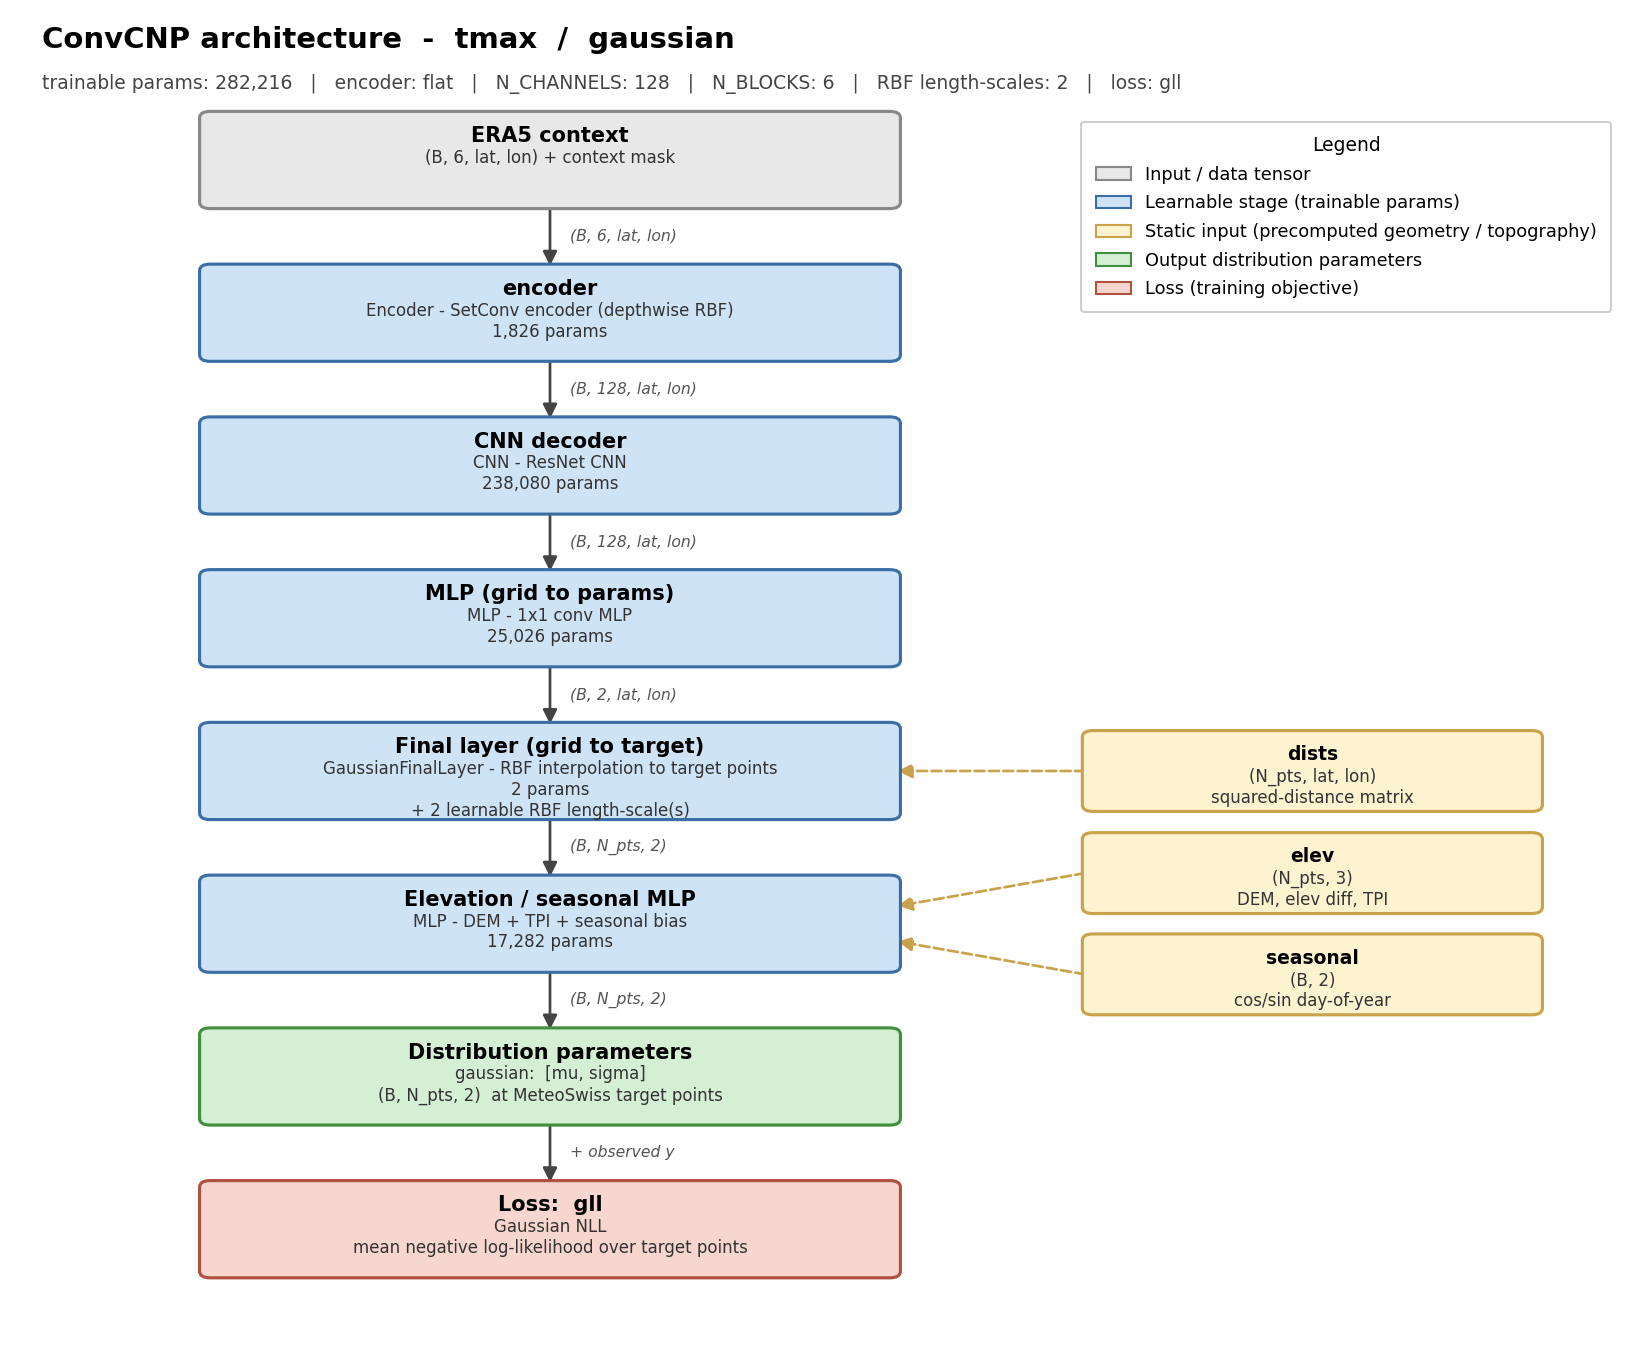
\includegraphics[width=0.45\textheight]{images/architecture/tmax-surface_architecture.png}
\caption[ConvCNP architecture of the surface-baseline model]{ConvCNP architecture for the surface-baseline temperature model (\tref{tab:data-context}). Atmospheric configurations differ only in the number of encoder input channels and the input grid resolution. The temperature and precipitation models differ depending on their configuration in the predictive distribution and the objective function.}
\label{fig:meth-architecture}
\end{figure}

\subsection{Encoder, CNN Processor, and RBF Final Layer}\label{subsec:meth-backbone}
In this part of the architecture, the model learns the relationships between the input channels and how to map them to the target points. The encoder processes the input context channels, which are stacked into a tensor $Z$ on their native grid. This tensor passes through the encoder, a depthwise set convolution that normalises each channel by its observation density, followed by a linear layer that lifts the channels to the working width of the CNN. The CNN backbone is a ResNet that learns the meteorological and spatial structure of the fields on the input grid. To simplify the use of different predictive distributions, the output distribution parameters are generated in a separate layer (MLP (grid to params)). The distribution parameters are then passed to a final layer that maps them from the input grid to the target points using RBF interpolation.

The RBF interpolation layer lets the model predict at arbitrary target points rather than only on the input grid. That is what downscaling needs, since the fine target locations do not align with the coarse lattice, and it is also what allows the model to be queried directly at station coordinates, as in \textcite{vaughan2022convcnp} or in \cref{ch:stations}.
The model learns for each parameter $k$ of the distribution (for example $\mu, \sigma$ for the Gaussian) its own length scale $\ell_k$ for the RBF kernel that is used to interpolate in 2D space the parameters from the input grid to the target points,
\begin{equation}
    \tilde{\theta}_k(x) \;=\; \sum_{i,j} h_k(g_{ij})\, \exp\!\left(-\frac{\lVert x - g_{ij} \rVert^{2}}{2\,\ell_k^{2}}\right),
\label{eq:rbf-interp}
\end{equation}
where $g_{ij}$ are the points of the input grid and $h_k(g_{ij})$ the gridded value of parameter $k$ produced by the previous layer. The target location $x$ enters only through its distance to the grid points, so the layer is tied to no fixed set of target locations and can be queried anywhere in the domain. Its output $\tilde{\theta}_k(x)$ is defined at the target points, but is still a smooth interpolation of the coarse field; the sub-grid terrain detail is added by the elevation MLP.
The calculation of the RBF kernel is a huge task because of the high number of target points and grid cells. To avoid memory issues within the GPU, the RBF kernel has to be  evaluated in chunks.

\subsection{Elevation MLP Correction}\label{subsec:meth-elev-mlp}

The elevation MLP, $\mathrm{MLP}_{\mathrm{elev}}$ in \eref{eq:convcnp-composition}, is used to add the terrain information to the model. The elevation MLP is a small MLP that takes the current distribution parameters together with the terrain features of the target points (elevation, elevation difference to the coarse model orography, TPI-500; \tref{tab:data-context}) together with the seasonal encoding, and outputs the corrected parameters of the predictive distribution directly,
\begin{equation}
    \theta(x) \;=\; \mathrm{MLP}_{\mathrm{elev}}\bigl(\,\tilde{\theta}(x) \oplus e(x) \oplus s\,\bigr),
\label{eq:elev-mlp}
\end{equation}
where $\oplus$ denotes concatenation: the three terrain features $e(x)$ and the two seasonal values $s$ are appended to the parameters $\tilde{\theta}(x)$ coming from \eref{eq:rbf-interp}. This gives seven inputs for temperature and eight for precipitation. The MLP returns a complete representative set of parameters, not merely an offset or bias added to $\tilde{\theta}(x)$.

This lets the model correct predictions that would otherwise be elevation agnostic, following \textcite{vaughan2022convcnp}, including seasonal effects such as differing lapse rates between summer and winter. Both the terrain and the seasonal encoding reach the model twice: coarsely, as scaffold channels processed by the encoder--CNN chain, and per target point, through the elevation MLP. This creates the link between the elevation seen for the meteorological input and the fine-grained per-point features including true elevation, TPI-500 and the elevation difference to the coarse model orography.

\section{Output Distributions}\label{sec:meth-distributions}

We study two separate target variables that behave differently. Daily maximum temperature at $2\,\mathrm{m}$ above ground is a continuous variable that is well modelled by a Gaussian distribution. Daily precipitation accumulation is more complex, as most days are dry and the wet days follow a skewed distribution. A Bernoulli--Gamma mixture is the standard parametric answer, used for precipitation density networks by \textcite{cannon2008berngamma} and for ConvCNP downscaling by \textcite{vaughan2022convcnp}; we adopt it here.

For both variables the model predicts the parameters of a distribution at each target point and day rather than a single value. Downscaling is ill-posed, one coarse field being compatible with many fine-scale outcomes, and a distribution keeps that ambiguity explicit; it also makes the probability of exceeding any threshold directly available and lets the prediction be checked for calibration.

Each distribution is factorised across target points (\sref{sec:bg-neural-processes}): \eref{eq:gauss-density} and \eref{eq:bg-density} are marginals at one point and day, not components of a joint distribution with a learned covariance. The predicted spread therefore describes that point alone and says nothing about its neighbours, and every score of \sref{subsec:meth-metrics} is accordingly a marginal score.

\subsection{Gaussian for Temperature}\label{subsec:meth-gaussian}

For temperature, this distribution is a Gaussian: the model outputs a mean $\mu$ and a standard deviation $\sigma$ at every target point, which define the density over the possible temperatures $y$,
\begin{equation}
    p(y) \;=\; \frac{1}{\sqrt{2\pi\sigma^{2}}} \exp\!\left(-\frac{(y - \mu)^{2}}{2\sigma^{2}}\right).
\label{eq:gauss-density}
\end{equation}
\fref{fig:meth-tmax-dist} illustrates the resulting density: one mean and one spread per target point and day.

\begin{figure}[H]
\centering
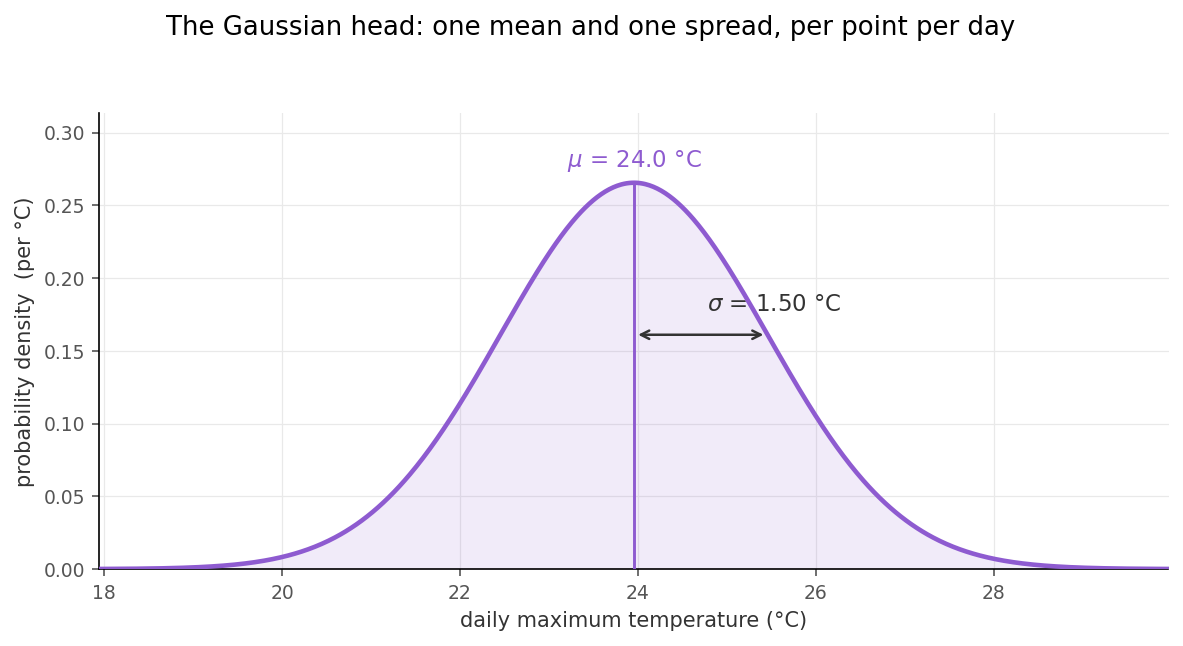
\includegraphics[width=0.9\textwidth]{images/16_tmax_distribution.png}
\caption[The Gaussian predictive distribution]{The Gaussian predictive density for a single target point and day. The model outputs the two parameters: the mean $\mu$ locates the distribution and the standard deviation $\sigma$ sets its width, shown here for $\mu = 24.0\,^{\circ}\mathrm{C}$ and $\sigma = 1.5\,^{\circ}\mathrm{C}$.}
\label{fig:meth-tmax-dist}
\end{figure}
\subsection{Bernoulli--Gamma for Precipitation}\label{subsec:meth-likelihoods}

Precipitation needs a different shape. Most days are exactly dry, $0\,\mathrm{mm}$, and the wet days follow a skewed, strictly positive distribution (\sref{subsec:data-coords}). Following \textcite{cannon2008berngamma} and \textcite{vaughan2022convcnp}, we therefore use a Bernoulli--Gamma mixture: $\rho$ is the probability that the day is wet, and $\alpha$ and $\beta$ are the shape and rate of a Gamma distribution for the amount of precipitation. Write $g(y; \alpha, \beta)$ for that Gamma density and $G(y; \alpha, \beta)$ for its cumulative distribution function. A wet day is scored by the probability of rain times the density of the amount, a dry day by the probability of staying dry,
\begin{equation}
    p(y) \;=\;
    \begin{cases}
        \rho \, g(y; \alpha, \beta) & y > 0 \text{ (wet)}, \\
        1 - \rho & y = 0 \text{ (dry)}.
    \end{cases}
\label{eq:bg-density}
\end{equation}
The three parameters are easiest to read as the probability of at least $t$ millimetres. For any threshold $t > 0$ the mixture of \eref{eq:bg-density} gives that probability in closed form,
\begin{equation}
    P(Y \geq t) \;=\; \rho \, \bigl(1 - G(t; \alpha, \beta)\bigr),
\label{eq:bg-exceedance}
\end{equation}
which reads directly: the day has to be wet, which costs $\rho$, and the amount then has to reach $t$. This exceedance probability is what the precipitation indices and skill scores later ask of the model (\sref{subsec:app-skill-precip}). \fref{fig:meth-precip-dials} visualises different shapes of possible output distributions. $\rho$ reweights the same wet body without changing its shape such that the gap to 1 at 0 mm is the probability of a dry day. $\beta$ changes how much precipitation accumulates once it does rain, stretching the curve to the right while the dry mass stays where it is. $\alpha$ changes the shape of a wet day: a given average is reached either through many small amounts or through fewer, heavier ones. The provided examples are realistic draws from a model output.

\begin{figure}[H]
\centering
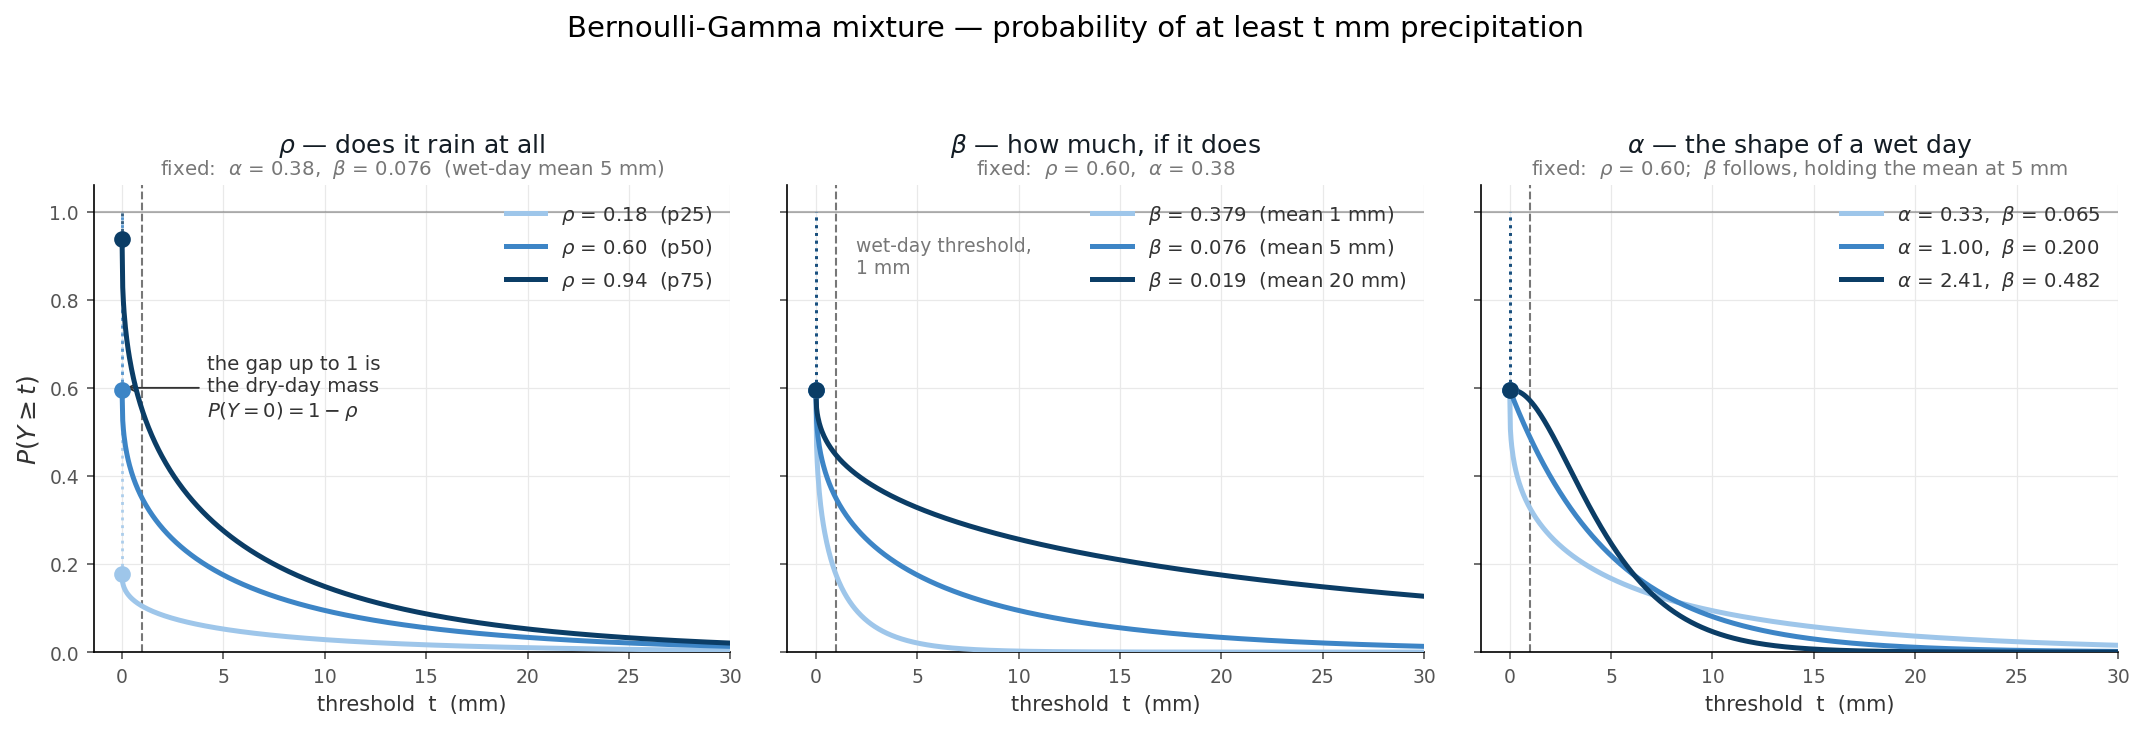
\includegraphics[width=\textwidth]{images/17_precip_wet_dry_day.png}
\caption[Bernoulli--Gamma distribution]{The Bernoulli--Gamma head read as the probability of at least $t$ millimetres, with one parameter turned per panel and the other two held constant. All parameter values are sampled from one of the model own outputs}

\label{fig:meth-precip-dials}
\end{figure}

\fref{fig:meth-precip-dials} reads the distribution at a single point and day; \sref{subsec:app-skill-precip} explains how these point-day distributions are pooled into the frequencies the results chapter actually reports.

\section{Training and Evaluation Setup}\label{sec:meth-training}

\subsection{Temporal $k$-Fold Cross-Validation and Hyperparameters}\label{subsec:meth-cv}

The models of this work are trained on the four years 2020--2023 and never see the year 2024, which is kept aside for the final evaluation. Within the training years, we use a temporal $k$-fold cross-validation with $k=5$: the days are split into five contiguous blocks of about $290$ days, and each fold trains on four blocks while the fifth is held out (\fref{fig:meth-cv-scheme}). The blocks are contiguous in time on purpose. Consecutive days share their weather, so a random split would place near-copies of training days into the held-out set and overstate the skill; a held-out block of many consecutive months has to be predicted from genuinely different periods.

\begin{figure}[H]
\centering
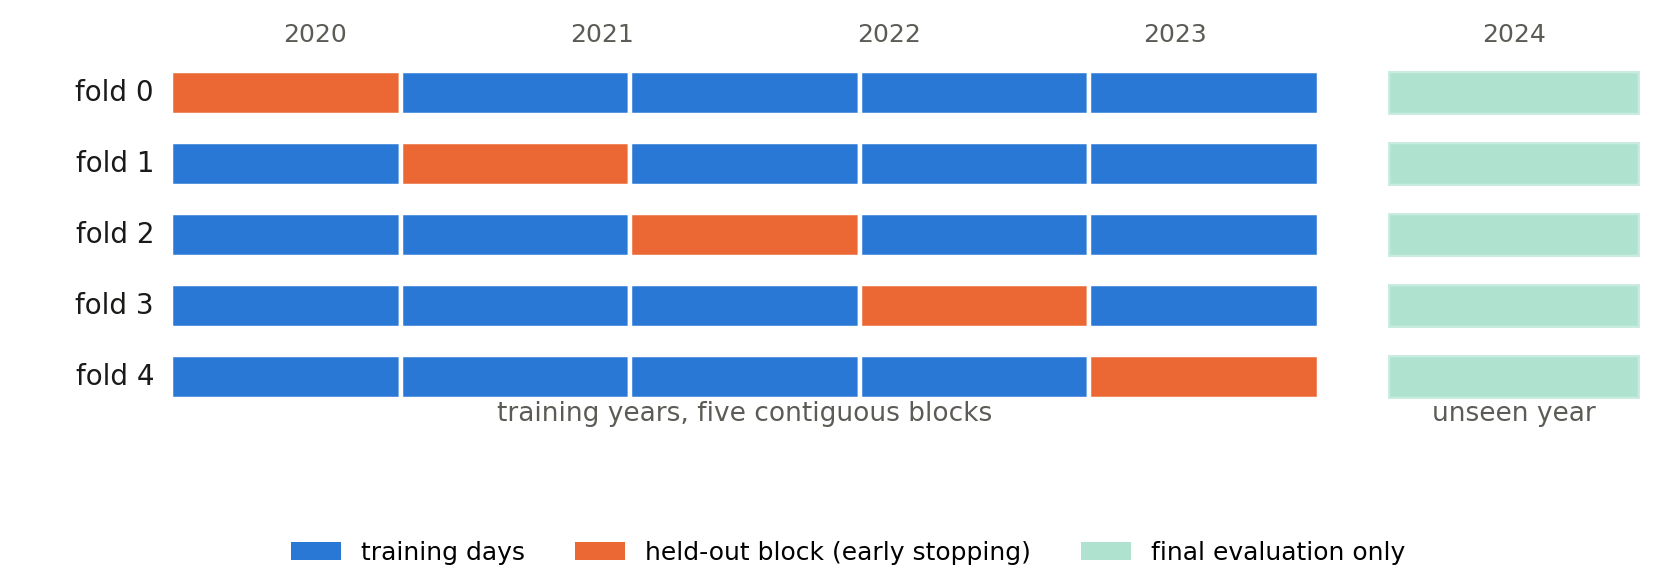
\includegraphics[width=0.9\textwidth]{images/cv_scheme.png}
\caption[Temporal cross-validation scheme]{The temporal $5$-fold scheme. Each fold trains on four contiguous blocks of 2020--2023 and holds out the fifth; the year 2024 is used for the final evaluation only.}
\label{fig:meth-cv-scheme}
\end{figure}

The training loop is standardised, and the hyperparameters it uses are collected in
\tref{tab:meth-training-setup}. They follow \textcite{vaughan2022convcnp} and the predecessor
pipeline rather than a tuning study of their own; beyond an early coarse screen of the
precipitation model, no hyperparameter search was run in this work.

The loop is identical for both variables; only the objective differs, and with it the stabilisation it needs, as the two subsections below state.


The five-fold split of \fref{fig:meth-cv-scheme} creates two deployment regimes: in the cross-validation evaluation each model predicts only the holdout block it never trained on, so every day is predicted exactly once by an independent model, whereas in all inference situation on unseen data the five trained models act together as an ensemble (\sref{sec:meth-inference}).

\subsection{Objective Functions}\label{objective}
The negative log-likelihood objectives follow \textcite{vaughan2022convcnp}. For the precipitation model, we extended the training with a CRPS-based objective function, used both from scratch and as a fine-tune of a converged likelihood model. The fine-tune is what earns the third run its place: ten of its epochs recover more of the held-out CRPS than thirty epochs of training on the CRPS from scratch (\sref{sec:app-precip-training}).

Whichever objective is used, it is evaluated over the Swiss domain alone. The input grid extends beyond the national border (\tref{tab:data-context}), but the loss is formed only at the MeteoSwiss target points that carry an observation: target values outside the analysis domain are missing, and every objective drops them before averaging. Of the $88\,800$ points of the temperature lattice, $46\,718$ ($53\,\%$) are inside Switzerland and enter the loss; the precipitation lattice contributes about $64\,\%$ of its $98\,050$ points. The exclusion happens at the loss and nowhere earlier. The context grid is never cropped, the full rectangular MeteoSwiss product grid is flattened into the target-point tensor with the outside-Switzerland points kept as \texttt{NaN} rather than removed, and the model's forward pass, the RBF final layer and the elevation MLP alike, predicts at every one of those points, including the ones with no observation. 
\subsubsection*{Temperature}\label{subsubsec:meth-train-tmax}

The temperature runs minimise the negative log-likelihood of the Gaussian of \eref{eq:gauss-density}, averaged over all target points and days of a batch,
\begin{equation}
    \mathcal{L}_{\mathrm{T}} \;=\; -\,\overline{\log p(y)} \;=\; \overline{\tfrac{1}{2}\log\bigl(2\pi\sigma^{2}\bigr) + \frac{(y - \mu)^{2}}{2\sigma^{2}}}.
\label{eq:gauss-ll}
\end{equation}
The targets enter in normalised units, $z$-scored with the statistics of the ERA5-Land $\mathrm{t2m\_max}$ field (\sref{subsec:data-coords}), so the objective sees values of order one. The Gaussian likelihood is well behaved throughout, and no further stabilisation is needed.

\subsubsection*{Precipitation}\label{subsubsec:meth-train-precip}

The precipitation runs train on raw millimetres: a $z$-score would push the exact zeros to negative values and destroy the point mass the Bernoulli--Gamma mixture is built on (\sref{subsec:data-coords}).

Two objectives are implemented and selected per run. The first is the negative log-likelihood of the mixture of \eref{eq:bg-density},
\begin{equation}
    \mathcal{L}_{\mathrm{P}} \;=\; -\,\overline{r\,\bigl(\log \rho + \log g(y; \alpha, \beta)\bigr) + (1-r)\log(1-\rho)},
\label{eq:bg-ll}
\end{equation}
with $y$ the observed accumulation, $\rho$ the predicted probability of a wet day, $\alpha$ and $\beta$ the predicted shape and rate of the Gamma body, and $r=1$ on wet days ($y>0$) and $r=0$ on dry days; the bar is the average over all target points and days of a batch.

The second objective is the CRPS of \eref{eq:crps}, which judges the whole predictive distribution instead of the density at the value that occurred. It has no closed form for the mixture, so it is estimated in the kernel form given by \textcite{gneiting2007scoring}, which writes the score as expected absolute differences and therefore needs only draws from the predictive distribution. Applied to the mixture, this leaves the dry outcome analytic and only the two Gamma expectations to sample, each from its own independent set of $25$ draws taken with the implicit reparameterisation of \textcite{figurnov2018implicit}, which is what carries the gradient to $\alpha$ and $\beta$. 

The CRPS objective is used either from scratch or to fine-tune a model first trained on the log-likelihood, and the same estimate is evaluated on the log-likelihood runs as well, so all precipitation runs share one CRPS curve (\sref{sec:app-precip-training}). Each fold keeps the checkpoint with the best held-out score under the objective it is trained on, and the gradient norm is clipped to $1$.

\tref{tab:meth-training-setup} collects the objectives and the default training setting they are trained with.

\begin{table}[htbp]
\centering
\caption[Objectives and the default training setting]{Objectives and the default training setting. If not stated otherwise, all models are generated along this line. The upper block is what differs between the variables and the three precipitation runs; the lower block is the default setting, used wherever a run states nothing else.}
\label{tab:meth-training-setup}
\scriptsize
\setlength{\tabcolsep}{4pt}
\newcommand{\rr}{\raggedright\arraybackslash}
\begin{tabular}{|>{\rr}p{1.9cm}|>{\rr}p{2.7cm}|>{\rr}p{2.7cm}|>{\rr}p{2.7cm}|>{\rr}p{2.7cm}|}
\hline
& \textbf{Temperature} & \textbf{Precipitation, NLL} & \textbf{Precipitation, CRPS} & \textbf{Precipitation, NLL then CRPS} \\
\hline
Distribution & Gaussian $(\mu, \sigma)$ & Bernoulli--Gamma $(\rho, \alpha, \beta)$ & Bernoulli--Gamma $(\rho, \alpha, \beta)$ & Bernoulli--Gamma $(\rho, \alpha, \beta)$ \\
\hline
Objective & Gaussian NLL, \mbox{\eref{eq:gauss-ll}} & mixture NLL, \mbox{\eref{eq:bg-ll}} & sampled CRPS, \mbox{\eref{eq:crps}} & mixture NLL, then sampled CRPS \\
\hline
Initialisation & random & random & random & warm start from the trained NLL model \\
\hline
Targets & Kelvin, $z$-scored with the ERA5 statistics & raw millimetres & raw millimetres & raw millimetres \\
\hline
Monte Carlo draws & --- & $25$, as a diagnostic only & $25$ per Gamma expectation & $25$ per Gamma expectation \\
\hline
Gradient clip & none & $1$ & $1$ & $1$ \\
\hline
Departure from the default & --- & --- & --- & learning rate $5 \cdot 10^{-5}$, at most $10$ epochs, patience $3$ \\
\hline
\multicolumn{5}{|l|}{\textit{Default training setting}} \\
\hline
Optimiser & \multicolumn{4}{>{\rr}p{\dimexpr 10.8cm+6\tabcolsep+3\arrayrulewidth\relax}|}{Adam, learning rate $5 \cdot 10^{-4}$, batches of $8$ days} \\
\hline
Schedule & \multicolumn{4}{>{\rr}p{\dimexpr 10.8cm+6\tabcolsep+3\arrayrulewidth\relax}|}{At most $30$ epochs, early stopping after $10$ epochs without improvement on the held-out block, best epoch kept\newline Extended training $60$ epochs, patience $20$} \\
\hline
Cross-validation & \multicolumn{4}{>{\rr}p{\dimexpr 10.8cm+6\tabcolsep+3\arrayrulewidth\relax}|}{Five temporal folds over 2020--2023, one model per fold (\sref{subsec:meth-cv})} \\
\hline
\end{tabular}
\end{table}

\FloatBarrier


\subsection{Metrics}\label{subsec:meth-metrics}

Because both models output a distribution rather than a single value (\sref{sec:meth-distributions}), the evaluation needs three kinds of measure: deterministic errors for the central prediction, proper scores for the whole predictive distribution, and skill scores that express either of the two against a reference built from the ERA5-Land fields. The reference is always evaluated on the same target points, days and aggregation level as the model it is compared with. Definitions are given in \sref{sec:app-metrics}.

Temperature (continuous, Gaussian) and precipitation (mixed discrete--continuous, Bernoulli--Gamma) require distinct approaches to evaluate the results. \tref{tab:meth-metrics-summary} lists and associates the metrics used. Throughout, $F$ denotes the predictive cumulative distribution function of whatever is being scored: the model's Gaussian or Bernoulli--Gamma at one target point and day, or the step function of a deterministic reference.

Every metric is scored in one of the two regimes of \sref{subsec:meth-cv} and the two are never
pooled: the \emph{CV holdout} uses a single fold with no ensembling, scoring each of the four training
years by the one fold that never saw it, while the \emph{2024 holdout} uses the five-fold ensemble on the
unseen year, normalised with training statistics. Within a regime the same metric is read at whichever
aggregation level answers the question at hand; pooled, per target point, per day, or per fold ; and
the level is stated wherever a number is quoted. \tref{tab:app-eval-regimes} sets out what each level
means and where the pooled and per-point forms of a metric differ.

\begin{table}[htbp]
    \centering
    \caption[Evaluation metrics at a glance]{The metrics reported in this work and the question each
    one answers. Var: \textbf{T}emperature, \textbf{P}recipitation. Ranges, optimal directions and the
    pooling recipe of every metric are given in \tref{tab:app-metrics-overview}.}
    \label{tab:meth-metrics-summary}
    \footnotesize
    \begin{tabular}{|>{\raggedright\arraybackslash}p{4.6cm}|>{\centering\arraybackslash}p{0.7cm}|>{\raggedright\arraybackslash}p{7.4cm}|}
        \hline
        \textbf{Metric} & \textbf{Var} & \textbf{Question it answers} \\
        \hline
        MAE, RMSE, bias & T, P & How far is the central prediction from the truth, and is the error systematic \\
        \hline
        CRPS & T, P & How good is the whole predictive distribution, not just its centre \\
        \hline
        CRPSS, MAE skill, BSS, RPSS & T, P & How much does the model add over interpolating the coarse field \\
        \hline
        R01, dry-day fraction, SDII, R10, P98 & P & Does the predicted rain behave physically: how often, how hard, and how extreme \\
        \hline
        PIT, standardised-error SD, coverage & T, P & Is the predicted uncertainty honest \\
        \hline
    \end{tabular}
\end{table}


The properties of this set that matter for reading \cref{ch:single-model} are set out together
with the definitions in \sref{sec:app-metrics}.
\section{Inference}\label{sec:meth-inference}

For inference all five folds (\sref{subsec:meth-cv}) predict every day and act together as an ensemble: the predicted mean is the average of the five means, and the predictive variance combines the average within-model variance with the spread between the five means, so disagreement between folds widens the predicted distribution,
\begin{equation}
    \mu_{\mathrm{ens}} \;=\; \frac{1}{K}\sum_{k=1}^{K} \mu_k,
    \qquad
    \sigma^{2}_{\mathrm{ens}} \;=\; \underbrace{\frac{1}{K}\sum_{k=1}^{K} \sigma_k^{2}}_{\text{within a fold}}
    \;+\; \underbrace{\frac{1}{K}\sum_{k=1}^{K} \bigl(\mu_k - \mu_{\mathrm{ens}}\bigr)^{2}}_{\text{between the folds}},
    \label{eq:fold-ensemble}
\end{equation}
with $K = 5$ folds. For precipitation, whose head has no single mean and spread, the ensemble averages the three Bernoulli--Gamma parameters over the folds.


\section{Feature Importance}\label{sec:meth-fi}

Whether the model learns physically meaningful relationships (\cref{ch:introduction}) cannot be read
off its weights, because the encoder mixes all channels immediately after its per-channel smoothing.  Therefore specialised techniques are needed to attribute the model's output to its inputs. The goal is to understand which input channels the model relies on most, and whether that reliance is physically plausible.

\subsection{Choosing the Attribution Method}\label{subsec:meth-fi-choice}
\tref{tab:meth-fi-methods} compares candidate attribution methods. Three requirements decide the suitable choice here: the result has to describe the trained model as a whole, it has to query the model itself rather than a substitute for it, and it has to be expressed as a loss of accuracy so that models can be compared with each other. Permutation importance with time as the permutation axis meets  all three and is the cheapest of them computationally. 

Two properties of the estimator bound what the resulting importances can support. A channel that does not vary in time is unchanged by a permutation along the day axis, so latitude, longitude and the coarse elevation score exactly zero by construction rather than by irrelevance; and what is measured is the loss of accuracy when a channel is destroyed, which is a statement about reliance and not about causation. The remaining limitations are set out in \sref{subsec:app-fi-limits}.

For reference LIME was also executed as a cross-check (\sref{subsec:app-fi-lime}). SHAP was implemented in the codebase but not systematically run on the models due to its high computational cost. It answers the same question at a multiple of the cost, however high correlation between inputs can lead to a bias of the attribution \cite{aas2021dependent}.

\begin{table}[htbp]
\centering
\caption[Feature importance method comparison]{Feature importance method comparison. Only ablation changes the model; the others query the trained one as a black box.}
\label{tab:meth-fi-methods}
\footnotesize
\setlength{\tabcolsep}{4pt}
\begin{tabular}{|p{1.5cm}|p{2.5cm}|p{2.5cm}|p{2.0cm}|p{2.0cm}|p{2.0cm}|}
\hline
\textbf{Method} & \textbf{What is perturbed} & \textbf{Attributed to} & \textbf{Scope} & \textbf{Cost} & \textbf{Role here} \\
\hline
Ablation \mbox{\cite{meyes2019ablation}} & the channel is removed and the model retrained & the error of a \emph{retrained} model & global & one training run per channel & not used \\
\hline
PFI \mbox{\cite{breiman2001rf}}, \mbox{\cite{fisher2019allmodels}} & the channel is scrambled across days & the error of \emph{this} model & global & $R$ inference passes per channel & primary \\
\hline
LIME \mbox{\cite{ribeiro2016lime}} & channels masked to their climatology, one day at a time & the model's own output & one day, spatially averaged & masks $\times$ days & cross-check \\
\hline
SHAP \mbox{\cite{lundberg2017shap}} & channels masked over coalitions & the error of \emph{this} model & global & ${\approx}10\times$ PFI & implemented, not run \\
\hline
\end{tabular}
\end{table}

\subsection{Permutation Feature Importance (PFI) on a Group of Channels}\label{subsec:meth-fi-groups}\label{subsec:meth-fi-pfi}

Permutation importance breaks the association between an input and the target and charges the model
for the accuracy it loses~\cite{breiman2001rf,fisher2019allmodels}. The
permutation axis chosen here is time: a channel keeps its fields but receives them shuffled, so on a given
day it carries a real field from another day while every other channel carries the day being
predicted. With $Z$ the context tensor, $L$ the
metric over all days and target points, and $Z^{(\pi, j)}$ that tensor with channel $j$ reordered
along the day axis,
\begin{equation}
I_j \;=\; \frac{1}{R} \sum_{r=1}^{R} \Bigl[\, L\bigl(Z^{(\pi_r,\, j)}\bigr) \;-\; L(Z) \,\Bigr],
\label{eq:pfi}
\end{equation}
so $I_j$ carries the units of the variable, and every permuted field remains one the atmosphere could
produce.

One channel at a time understates correlated
channels~\cite{hooker2021unrestricted}, since neighbouring levels and adjacent
hours are highly correlated. Permuting a whole group at once, with one
day permutation shared across its channels, borrows a complete profile from a single other day
instead. Each channel belongs to one group of each grouping in \tref{tab:meth-fi-groups}. A group
importance is therefore always measured by permuting all the channels of a group at once. This is not equivalent to just summing single channel importances.
The grouped view carries the argument throughout this work and the per-channel view
only shows where the feature importance sits inside a group.

\begin{table}[htbp]
\centering
\caption[The three channel groupings]{The three groupings, with the number of channels a single group collects in each configuration. Only the variable grouping partitions the whole input; the level and hour groupings omit the channels that sit on no pressure surface or at no sampling hour, such as the scaffold.}
\label{tab:meth-fi-groups}
\footnotesize
\setlength{\tabcolsep}{4pt}
\begin{tabular}{|p{1.5cm}|p{2.0cm}|p{3.3cm}|p{1.0cm}|p{1.0cm}|p{1.4cm}|p{0.9cm}|p{1.0cm}|}
\hline
\textbf{Grouping} & \textbf{Groups} & \textbf{One group collects} & \textbf{atm} & \textbf{+wind} & \textbf{+anchors} & \textbf{sfc} & \textbf{sfc-tp} \\
\hline
Variable & $z$, $t$, $q$ & one physical variable, at every level and every hour & 30 & 30 & 30 & --- & --- \\
\hline
& $u$, $v$ & the wind components, in the extended set only & --- & 30 & --- & --- & --- \\
\hline
& $t2m$, $tp$ & one surface anchor, at every hour & --- & --- & 5 & --- & --- \\
\hline
& data & the coarse daily $\mathrm{t2m\_max}$ field (the target's own coarse field in the temperature runs) & --- & --- & --- & 1 & 1 \\
\hline
& tp & the ERA5-Land daily precipitation total, in the surface precipitation run only & --- & --- & --- & --- & 1 \\
\hline
& scaffold & latitude, longitude, the two seasonal channels and the coarse elevation & 5 & 5 & 5 & 5 & 5 \\
\hline
Level & $1000$, $925$, $850$, $700$, $500$, $300\,\mathrm{hPa}$ & every variable on that pressure surface, at every hour & 15 & 25 & 15 & --- & --- \\
\hline
Hour & $00$, $06$, $12$, $15$, $18$~UTC & every variable at every level at that hour, and the anchors where present & 18 & 30 & 20 & --- & --- \\
\hline
\multicolumn{3}{|l|}{\textbf{Channels in the model} (the variable groups summed)} & $95$ & $155$ & $105$ & $6$ & $7$ \\
\hline
\end{tabular}
\end{table}

\subsection{Interpretation of Feature Importances}\label{subsec:meth-fi-reported}

Degradation can be measured with the metrics of \tref{tab:meth-fi-setup} over every day and target
point, so an importance is a change in the annual, domain-wide error. The precipitation CRPS is
absent because it must be sampled for the mixture, and an importance is a difference of two scores,
so the introduction of sampling would introduce additional variance. Reliance is defined only relative to the distribution the model is
evaluated under~\cite{fisher2019allmodels}: evaluated on training data, an importance measures what
the model uses; evaluated on holdout data, it measures what it uses that also generalises to unseen
days.
The evaluation occurs on the 2024 holdout year and the baseline of \eref{eq:pfi} is therefore the holdout-year error reported in
\cref{ch:single-model}.

\begin{table}[htbp]
\centering
\caption[Configuration of the feature-importance study]{Configuration of the feature-importance study. The same settings are used for every trained configuration, so the results are comparable across runs.}
\label{tab:meth-fi-setup}
\footnotesize
\begin{tabular}{|p{3.6cm}|p{5.2cm}|p{5.2cm}|}
\hline
& \textbf{Temperature} & \textbf{Precipitation} \\
\hline
Scored period & \multicolumn{2}{p{10.8cm}|}{The holdout year 2024, all $366$ days, with all five folds ensembled and the normalisation frozen at training, the deployment regime of \sref{sec:meth-inference}. No fold saw these days, so the importances are out-of-sample} \\
\hline
Target points & $88\,800$ & $98\,050$ \\
\hline
Metrics computed & MAE, Gaussian NLL, CRPS $[^{\circ}\mathrm{C}]$ & MAE $[\mathrm{mm}]$, Bernoulli--Gamma NLL \\
\hline
Metric reported & MAE $[^{\circ}\mathrm{C}]$ & MAE $[\mathrm{mm}]$ \\
\hline
PFI & \multicolumn{2}{p{10.8cm}|}{Run on every configuration. $5$ permutation repeats, per channel // per group; groupings by variable, pressure level and hour} \\
\hline
LIME & \multicolumn{2}{p{10.8cm}|}{Run on every configuration. $4$ representative days $\times$ $1000$ channel masks; ridge penalty $1$, kernel width $0.25$ (\sref{subsec:app-fi-lime})} \\
\hline
SHAP & \multicolumn{2}{p{10.8cm}|}{Implemented, not run} \\
\hline
\end{tabular}
\end{table}

Some limitations bound what these importances support; they are set out in
\sref{subsec:app-fi-limits}.

\FloatBarrier
\subsection{Computational Cost}\label{subsec:meth-cost}

The model is small in weights and expensive in use. The configurations range from $282\,000$ to
$325\,000$ parameters, $1.1$ to $1.3\,\mathrm{MB}$ in single precision. The cost is set by the tens of thousands of target points
rather than by the network. The elevation MLP is where it accumulates: it runs once per target point
and never sees the input grid, and it accounts for most of the arithmetic on both grids
(\fref{fig:meth-cost-ops}). Underneath it the distance matrix holds a fixed allocation that is far
larger on the surface grid than on the atmospheric one, which is why the atmospheric configuration
is the cheaper of the two in memory as well as in operations despite carrying many more input
channels (\fref{fig:meth-cost-ops}, \fref{fig:meth-cost-mem}).

In practice a single mid-range GPU is sufficient: at the batch size of $8$ used here the forward
pass peaks below $2\,\mathrm{GB}$ (\fref{fig:meth-cost-mem}), the backward pass raises the full
training step to just below $2.2\,\mathrm{GB}$, and inference roughly halves that, so both fit on consumer hardware,
while a server allows several configurations to be trained at once. Should the cost ever become
binding, the easiest levers are a narrower elevation MLP, an RBF kernel restricted to the grid cells
within a few length scales of each target point, or a distance matrix kept in reduced numerical
precision.


\begin{figure}[H]
    \centering
    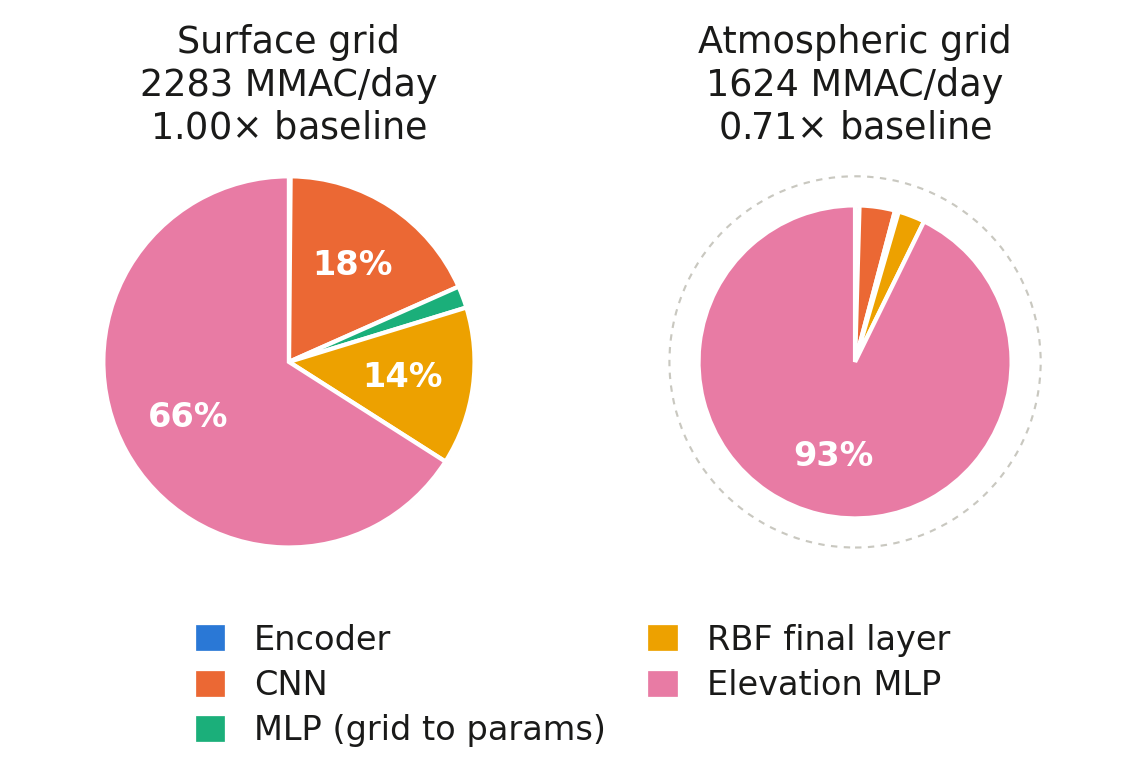
\includegraphics[width=0.75\textwidth]{images/component_cost_ops.png}
    \caption[Computational cost per component]{Computational cost per component: multiply-accumulate operations of one day, in millions, split into the architectural components.}
    \label{fig:meth-cost-ops}
\end{figure}

\begin{figure}[H]
    \centering
    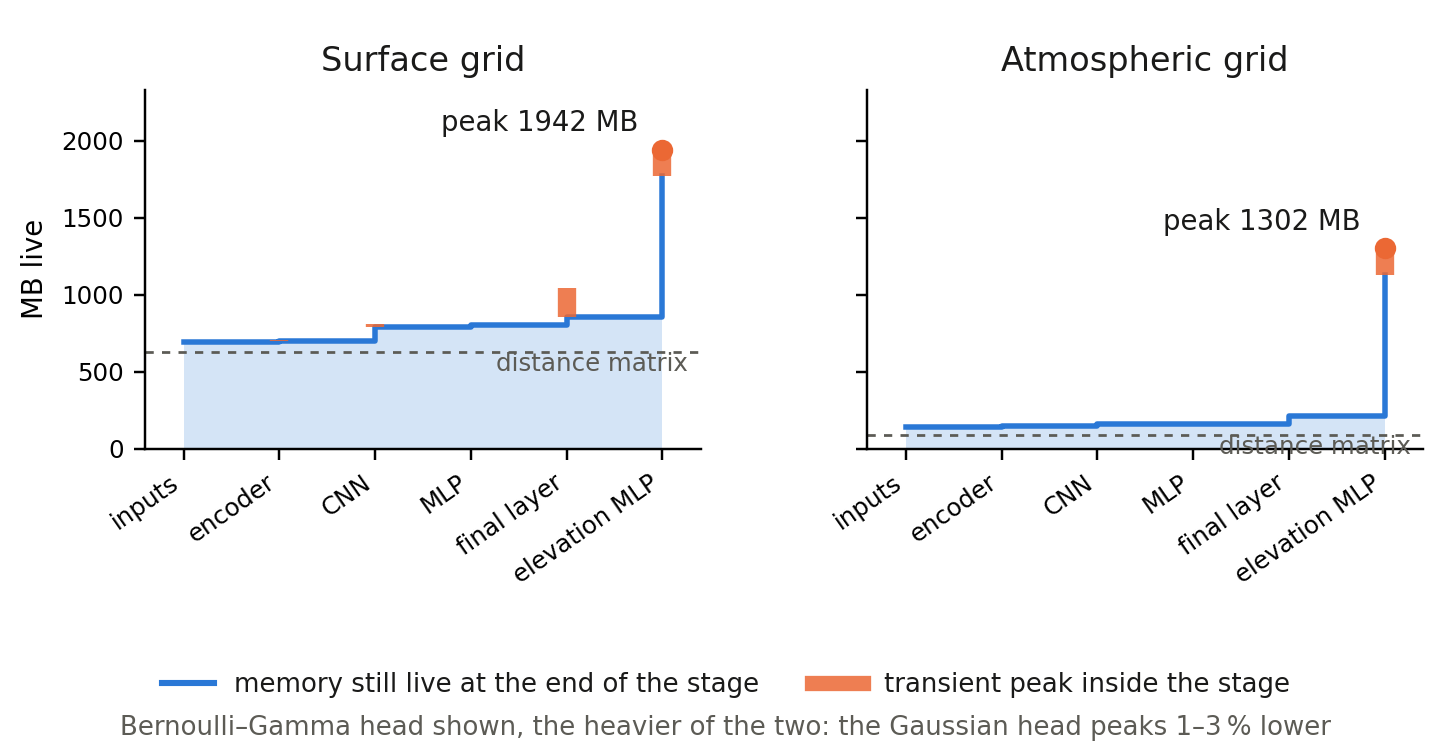
\includegraphics[width=0.86\textwidth]{images/component_cost_mem_profile.png}
    \caption[Memory through a training forward pass]{Memory estimation live at each stage of a training forward pass of the Bernoulli--Gamma configurations, the heavier of the two output heads, at the batch of eight days used in this work, with the transient inside each stage drawn above it. The peak is a moment inside a single stage, not a sum over stages.}
    \label{fig:meth-cost-mem}
\end{figure}

\FloatBarrier

Everything set out above is held fixed in what follows. The input set and the objective are the
two axes \cref{ch:single-model} varies.
